


\chapter{Electron Inertial Effects}
  \label{ch_inertia}

As laid out in \cref{ch_model}, Tuna resolves neither parallel currents nor parallel electric fields. This is unfortunate; parallel electric fields generated by kinetic and inertial \Alfven waves (including fundamental field line resonances\cite{rankin_1999,tikhonchuk_2000}) are a topic of particular interest in the study of auroral particle precipitation. 

Parallel currents and electric fields can be added to Tuna through the consideration of electron inertial effects in \ohmlaw:
\begin{align}
  0 &= \sz E_z - J_z & \text{becomes} & & \frac{1}{\nu} \ddt J_z &= \sz E_z - J_z
\end{align}

With the addition of the electron inertial term, it is necessary to track the parallel current independent of the parallel electric field\footnote{The parallel current $J_z$ is defined on the same points of the Yee grid as $E_z$. It is offset in time by half of a time step. }. Solving by integrating factors\footnote{The integrating factors technique is laid out explicitly for \amplaw in \cref{sec_eqns}. } gives
\begin{align}
  J_3 &\assign J_3 \, \exp \arg{ - \nu \dt } + \dt \, \frac{n e^2}{\me} E_3 \, \exp \arg{ -\nu \tfrac{\dt}{2} }
\end{align}

From there, the parallel electric field can be updated directly; \cref{e3_final} is replaced by the following: 
\begin{align}
  E_3 &\assign E_3 + c^2 \dt \, \lr{ g_{31} F^1 + g_{33} F^3 } - \frac{\dt}{\ez} J_3
\end{align}

The present section explores the complications that arise from the addition of the electron inertial term to \ohmlaw, as well as a few results that may be gleaned despite those complications. Notably --- for reasons discussed in \cref{sec_lengths} --- the results presented in \cref{ch_results} do not make use of the electron inertial term. 

Inertial effects have been considered in previous numerical work, such as by Lysak and Song in 2001\cite{lysak_2001}, but never at the global scale. Lysak and Song considered waves in the ionospheric \Alfven resonator, with frequencies of hundreds of \si{\mHz}. Their work did not account for the effects of the dipolar geometry, such as differenced that might arise between poloidal and toroidal resonances. In fact, in that work, circular polarization (essentially a superposition of poloidal and toroidal modes) was noted to be a promising avenue for future work. 

% -----------------------------------------------------------------------------
% -----------------------------------------------------------------------------
% -----------------------------------------------------------------------------
\section{The Boris Factor}
  \label{sec_boris}

With the addition of the electron inertial term, a cyclical dependence appears between \amplaw and \ohmlaw:
\begin{align}
  \ddt E_z &\sim -\frac{1}{\ez} J_z &
  & \text{and} & 
  \ddt J_z &\sim \frac{n e^2}{\me} E_z &
  & \text{so} &
  \frac{ \partial^2 }{ \partial t^2 } E_z &\sim -\op^2 E_z
\end{align}

That is, electron inertial effects come hand in hand with the plasma oscillation. 

\begin{figure}[!htb]
    \centering
    \includegraphics[width=\textwidth]{figures/op.pdf}
    \caption[Plasma Frequency Profile]{
      The plasma frequency reaches a peak value just under \SI{e6}{\Hz} near the equator. Outside the plasmasphere, its value is closer to \SI{e4}{\Hz}, which is still not well-resolved by Tuna's usual time step.  
    }
    \label{fig_op}
\end{figure}

As mentioned in \cref{ch_math} and shown in \cref{fig_op}, plasma oscillation is quite fast --- several orders of magnitude smaller than Tuna's time step as determined in \cref{sec_coords} (\about\SI{10}{\us}). This poses a conundrum. At Tuna's usual time step, the plasma oscillation becomes unstable within seconds\footnote{For stability, $\op \dt < 1$ is necessary. }. On the other hand, reducing the time step by three orders of magnitude to resolve the plasma oscillation is computationally infeasible; a run slated for an hour would require six weeks to complete. 

As it happens, this problem can be solved by artificially increasing the parallel electric constant above its usual value of \ez. Doing so lowers both the speed of light and the plasma frequency within the simulation. 

This technique --- and others like it --- has been widespread in numerical modeling since it was presented by Boris in 1970\cite{boris_1970}. The following paraphrases an argument by Lysak and Song\cite{lysak_2001}, outlining its validity specifically in the case of electron inertial effects. 

Supposing that the current and electric field are oscillating at frequency $\omega$, the parallel components of \amplaw and \ohmlaw can be written
\begin{align}
  - i \omega \ez E_z &= \oomz \lr{ \, \curl{B} \, }_z - J_z & - \frac{i \omega}{\nu} J_z &= \sz E_z - J_z
\end{align}

Then, eliminating the current, the parallel electric field can be related to the curl of the magnetic field by\footnote{From \cref{def_basics}, $c^2 \equiv \frac{1}{\mz \ez}$ and $\sz \equiv \frac{n e^2}{\me \nu}$ and $\op^2 \equiv \frac{n e^2}{\me \ez}$. }
\begin{align}
  \label{boris_criterion}
  \lr{ 1 - \frac{\omega^2 - i \nu \omega}{\op^2} } E_z &= \frac{c^2}{\op^2} \lr{ \nu - i \omega } \lr{ \, \curl{B} \, }_z
\end{align}

In \cref{boris_criterion}, $\frac{c}{\op}$ is the electron inertial length. While the speed of light and the plasma frequency each depend on \ez, their ratio does not. This allows an estimation of how much the model should be affected by an artificially-large electric constant (and thus an artificially-small plasma frequency). So long as $\frac{\omega^2 - i \nu \omega}{\op^2}$ remains small compared to unity, the model should behave faithfully. 

For waves with periods of a minute or so, even perhaps-implausibly large Boris factors are allowed; for example, increasing \ez by a factor of \num{e6} gives $\left| \frac{\omega^2 + i \omega \nu}{ \op^2 } \right| \lesssim 0.01$. %In some places, this causes the speed of light to fall below the \Alfven speed; R{\"o}nnmark\cite{ronnmark_2000} terms this behavior ``anisotropic vacuum.''

%\todo{Generalized \ohmlaw, in case we decide we need it. Could talk through why all of the other terms are OK to neglect.  
%\begin{align}
%  \vec{E} + \vec{U} \! \times \! \vec{B} & = 
%  \eta \vec{J} + \tfrac{\me}{n e^2} \lrb{
%    \tfrac{\partial}{\partial t} \vec{J} + \nabla \cdot \lr{ 
%      \vec{J} \, \vec{U} + \vec{U} \,\vec{J} +
%      \tfrac{1}{n e} \vec{J} \, \vec{J} } } +
%  \tfrac{1}{n e} \vec{J} \! \times \! \vec{B} -
%  \tfrac{1}{n e} \div{ \vec{P_e} }
%\end{align}
%}

% -----------------------------------------------------------------------------
% -----------------------------------------------------------------------------
% -----------------------------------------------------------------------------
\section{Parallel Currents and Electric Fields}
  \label{sec_jz}

As discussed in \cref{sec_implications}, parallel electric fields in this regime are expected to be six or more orders of magnitude smaller than the perpendicular electric fields. Numerical results show general agreement: in \cref{fig_electric_field_snapshots}, the parallel electric field appears comparable to its perpendicular counterparts only after its been scaled up by six orders of magnitude. 
\begin{figure}[!htb]
    \centering
    \includegraphics[width=\textwidth]{figures/electric_field_snapshots.pdf}
    \caption[Electric Field Snapshots]{
      Parallel electric fields are smaller than perpendicular electric fields by about six orders of magnitude. As a result, parallel electric fields do not contribute significantly to $\curl{E}$ in \farlaw. 
    }
    \label{fig_electric_field_snapshots}
\end{figure}

As such, the inclusion of electron inertial effects does not appreciably impact the simulation's gross behavior; in \farlaw, \curl{E} is essentially unaffected. Side by side snapshots of the magnetic fields in runs carried out with and without electron inertial effects are not visibly distinguishable\footnote{In a sense, this is reassuring. It ensures that the present section does not cast doubt on the results presented in \cref{ch_results}, where electron inertial effects are neglected. } (not shown). 

Even if there is no significant feedback through \farlaw, it's informative to consider the structures that arise in parallel currents and electric fields driven by perturbations in the ring current. For example, in \cref{fig_electric_field_snapshots}, the parallel electric field perturbation (with maxima near the ionosphere) exhibits the opposite harmonic structure to the perpendicular electric field components (which peak near the equator). 

\begin{figure}[!htb]
    \centering
    \includegraphics[width=\textwidth]{figures/slice_100km.pdf}
    \caption[Current and Poynting Flux at \SI{100}{\km}]{
      Four runs are shown above, one per row, with azimuthal modenumbers of 1, 4, 16, and 64. Columns show slices at \SI{100}{\km} of the real parallel current, poloidal Poynting flux, imaginary current, and toroidal Poynting flux respectively. The similarity visible across columns suggests that the real parallel current follows the poloidal Poynting flux, while the imaginary parallel current follows the toroidal Poynting flux (the toroidal fields are imaginary). At least, this is the case in regions of significant Hall conductivity. 
    }
    \label{fig_slice_100km}
\end{figure}

At low altitude, the Hall conductivity muddles the poloidal and toroidal electric fields. In this region, as shown in \cref{fig_slice_100km}, parallel currents coincide with strong Poynting flux. The imaginary component of the current lines up with the toroidal Poynting flux (which comes from imaginary $E_x$ and imaginary $B_y^*$), while the real current lines up with the poloidal Poynting flux ($E_y$ and $B_x^*$ are real)\footnote{As mentioned in \cref{ch_model}, poloidal field components are in practice overwhelmingly real, indicating that they coincide azimuthally with the (real) driving. Toroidal components are overwhelmingly imaginary, which corresponds to an azimuthal offset. }. 

Four runs are shown in \cref{fig_slice_100km}, one per row, with azimuthal modenumbers 1, 4, 16, and 64. The first and third columns show the real and imaginary components of the parallel current respectively, in units of \si{\uA/\m\squared}, sliced at an altitude of \SI{100}{\km}, the edge of the simulation domain. The second and fourth columns are the poloidal and toroidal Poynting flux respectively, in units of \si{\mW/\m\squared}. Latitude is shown on the vertical axis, and time on the horizontal axis. 

At higher altitude, where the Hall conductivity is small, parallel current is associated only with the toroidal mode. \cref{fig_slice_1000km} shows data from the same runs as \cref{fig_slice_100km}, arranged in the same way, but the values are taken at an altitude of \SI{1000}{\km} instead of \SI{100}{\km}. 

In \cref{fig_slice_1000km}, as in \cref{fig_slice_100km}, the imaginary component of the parallel current (third column) coincides more or less with the toroidal Poynting flux (fourth column). However, the real component of the parallel current (first column) is vanishingly small, even when the poloidal Poynting flux (second column) is strong. 

\todo{Is this expected? Tikhonchuk\cite{tikhonchuk_2000} looks specifically at the toroidal mode when considering shear \Alfven waves. Does the poloidal mode count as compressional even when it's guided? In his 2001 paper, Lysak\cite{lysak_2001} talks about how circularly-polarized waves might be interesting. That would be a superposition of the poloidal and toroidal modes, right? In that paper, he's looking at modes with frequencies of \SI{1}{\Hz} or so, in the context of the IAR. Lysak and Song's 2003 paper\cite{lysak_2003} looks at the toroidal mode, also in the IAR (?). }

Notably, the Poynting flux waveforms are rectified --- they primarily carry energy Earthward. The current, on the other hand, alternates between upward and downward flow. This effect presumably arises because the current is a linear quantity while the Poynting flux is quadratic: the electric and magnetic fields that make it up oscillate in phase, so their product is positive even when they are negative. 

\begin{figure}[!htb]
    \centering
    \includegraphics[width=\textwidth]{figures/slice_1000km.pdf}
    \caption[Current and Poynting Flux at \SI{1000}{\km}]{
      The above figure shows the same runs as \cref{fig_slice_100km}, except that the slices are taken at an altitude of \SI{1000}{\km} instead of \SI{100}{\km}. Morphological similarities are still evident between the imaginary parallel current and the toroidal Poynting flux. However, without the Hall conductivity to couple the modes, the poloidal mode does not appear to carry significant current along the field line. 
    }
    \label{fig_slice_1000km}
\end{figure}

The magnitude of the parallel current tops out over \SI{1}{\uA/\m\squared}, just shy of the up-to-tens of \si{\uA/\m\squared} inferred from ground observations and seen in situ\cite{carlson_1998,karlsson_1996,samson_1996}. 

It's also possible to consider the effect of parallel currents and electric fields on the ionosphere's energy budget, per Poynting's theorem:
\begin{align}
  \ddt u &= -\div{E} - \vec{J} \cdot \vec{E}
\end{align}

\begin{figure}[!htb]
    \centering
    \includegraphics[width=\textwidth]{figures/power_density.pdf}
    \caption[Power Density at the Ionosphere]{
      While field-aligned currents can be of significant size, they are not particularly good at depositing energy in the ionosphere. Energy deposited by the Poynting flux matches closely with Joule dissipation from the perpendicular currents, while $J_z E_z$ is smaller by several orders of magnitude. 
    }
    \label{fig_power_density}
\end{figure}

As shown in \cref{fig_power_density}, little energy transfer in the ionosphere is mediated by perpendicular components of the Poynting flux. The parallel component of $\vec{J} \cdot \vec{E}$ is comparably unimportant. The energy deposited in the ionosphere by the Poynting flux matches closely with the energy lost to Joule dissipation --- as it should, to conserve energy --- but according to the model, parallel currents and electric fields do not contribute significantly. 

%\todo{Parallel electric fields, supposedly, only appear at high altitude. \cite{marklund_1997,carlson_1998}. }

%\todo{Integrate up a parallel electric field to see the potential difference. Compare to the relation seen by \cite{olsson_1996}, $J_\parallel \sim \Psi_\parallel$ by a proportionality constant of \SIrange{e-8}{e-10}{\S/\meter\squared}. }

% -----------------------------------------------------------------------------
% -----------------------------------------------------------------------------
% -----------------------------------------------------------------------------
\section{Inertial Length Scales}
  \label{sec_lengths}

It's not quite fair to compare the parallel and perpendicular contributions to \curl{E} as is done in \cref{sec_jz}. Perpendicular electric fields are on the order of \SI{1}{\mV/\m}, with wavelengths on the order of \SI{e5}{\km}; they cause magnetic fields to change at a rate of around \SI{0.1}{\nT/\s}. Parallel electric fields, closer to \SI{e-6}{\mV/\m}, would need to vary over length scales of \SI{0.1}{\km} to match with that. 

Such scales are believable. The characteristic length scale of the plasma oscillation is the electron inertial length, $\frac{c}{\op}$, which is on the order of \SI{1}{\km} in the auroral ionosphere and \SI{0.1}{\km} in the low-altitude plasmasphere. However, Tuna's usual grid doesn't resolve structures so fine; its resolution bottoms out closer to \SI{10}{\km}. That is, with the inclusion of electron inertial effects, Tuna's grid is too coarse to resolve all of the waves expected to be present. The model is prone to instability as a result. 

\cref{fig_inertial_length} shows a run with perpendicular resolution smaller than the electron inertial length, side by side with an analogous run on the usual grid. In order to carry out the inertial-scale run, several concessions were made to computational cost. The run simulates only a duration of \SI{100}{\s} (other figures in the present chapter, and those in \cref{ch_results}, show \SI{300}{\s}), and the grid covers only the auroral latitudes from $L=5$ to $L=7$. 

\begin{figure}[!htb]
    \centering
    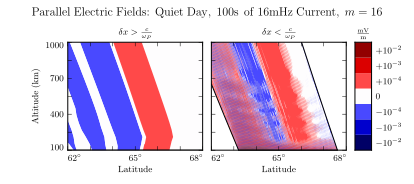
\includegraphics[width=\textwidth]{figures/inertial_length.pdf}
    \caption[Parallel Electric Fields by Perpendicular Grid Resolution]{
      The parallel electric field develops significant structure when the perpendicular grid resolution is smaller than the electron inertial length. Unfortunately, such runs are prohibitively expensive. The subplot on the right --- which still fails to resolve wave structure properly --- represents a 100-fold increase in computational time. 
    }
    \label{fig_inertial_length}
\end{figure}

Even so, the run presents a significant computational expense. Spread over 16 cores, a \SI{100}{\s} run on Tuna's usual grid takes well under an hour. The inertial-scale run barely finished in 96 hours, the cutoff at the Minnesota Supercomputing Institute\footnote{Runtime goes as the inverse square of grid resolution. Not only does finer resolution require more grid cells, but it also gives rise to proportionally smaller crossing times, imposing a smaller time step. }.

The snapshot shown in \cref{fig_inertial_length} uses a perpendicular grid resolution of \SI{0.7}{\km} at the Earthward edge, which just satisfies the Nyquist rate for the minimum inertial length of \SI{1.7}{\km}. It's still too coarse. There is clearly some small-scale structure developing in the ionosphere, but it's not well resolved. The large number of ``wigglies'' portends an imminent crash. 


% -----------------------------------------------------------------------------
% -----------------------------------------------------------------------------
% -----------------------------------------------------------------------------
\section{Discussion}

The present chapter is a proof of concept: the addition of electron inertial effects to Tuna presents a promising first-principles-based approach to the investigation of parallel currents and electric fields associated with field line resonances. Electric fields arise which are consistent in magnitude with those predicted by the dispersion relation, and parallel currents fall within an order of magnitude or so of observed values, even when inertial length scales are not properly resolved. 

Results in \cref{sec_jz} suggest a disparity between poloidal and toroidal FLRs in terms of the parallel current response. At low altitude, where the two modes are directly coupled by the Hall conductivity, both seem to be accompanied by parallel currents. However, in regions of low Hall conductivity, parallel currents appear to preferrentially accompany toroidal waves. The cause is unclear, and a topic worthy of future investigation. 

Future work in this vein may also consider the scales and structures that arise in regions of parallel current. For example, one might consider the relationship between the dynamic height-integrated potentials and the accompanying parallel currents, specifically with respect to the Knight Relation\cite{knight_1973}. Inertial effects could furthermore be accompanied by test particles, in order to gauge the properties of particle precipitation that could accompany global \Alfven{}ic potential structures. 

Unfortunately, simulations are prone to instability when inertial length scales are not properly resolved. And, at least at present, resolving those scales poses a prohibitive computational expense. For this reason, the consideration of inertial effects is limited to the present chapter; results in \cref{ch_results} make use of the core version of Tuna presented in \cref{ch_model}, which does not include the effects of electron inertia. 

Notably, the addition or omission of parallel currents and electric fields does not appear to significantly alter the behavior of perpendicular electric fields or magnetic fields. Because the parallel electric fields are relatively small, $\curl{E}$ is essentially unaffected by their inclusion. 







